\hypertarget{pop3-ux6536ux53d6ux90aeux4ef6}{%
\subsection{POP3 收取邮件}\label{pop3-ux6536ux53d6ux90aeux4ef6}}

SMTP 用于发送邮件,如果要收取邮件呢?

收取邮件就是编写一个 \textbf{MUA} 作为客户端,从 \textbf{MDA}
把邮件获取到用户的电脑或者手机上。收取邮件最常用的协议是 \textbf{POP}
协议,目前版本号是 3,俗称 \textbf{POP3}。

Python 内置一个\texttt{poplib}模块,实现了 POP3
协议,可以直接用来收邮件。

注意到 POP3
协议收取的不是一个已经可以阅读的邮件本身,而是邮件的原始文本,这和 SMTP
协议很像,SMTP 发送的也是经过编码后的一大段文本。

要把 POP3
收取的文本变成可以阅读的邮件,还需要用\texttt{email}模块提供的各种类来解析原始文本,变成可阅读的邮件对象。

所以,收取邮件分两步:

第一步:用\texttt{poplib}把邮件的原始文本下载到本地;

第二部:用\texttt{email}解析原始文本,还原为邮件对象。

\hypertarget{ux901aux8fc7-pop3-ux4e0bux8f7dux90aeux4ef6}{%
\subsubsection{通过 POP3
下载邮件}\label{ux901aux8fc7-pop3-ux4e0bux8f7dux90aeux4ef6}}

POP3 协议本身很简单,以下面的代码为例,我们来获取最新的一封邮件内容:

\begin{pythoncode}
import poplib

# 输入邮件地址, 口令和POP3服务器地址:
email = input('Email: ')
password = input('Password: ')
pop3_server = input('POP3 server: ')

# 连接到POP3服务器:
server = poplib.POP3(pop3_server)
# 可以打开或关闭调试信息:
server.set_debuglevel(1)
# 可选:打印POP3服务器的欢迎文字:
print(server.getwelcome().decode('utf-8'))

# 身份认证:
server.user(email)
server.pass_(password)

# stat()返回邮件数量和占用空间:
print('Messages: %s. Size: %s' % server.stat())
# list()返回所有邮件的编号:
resp, mails, octets = server.list()
# 可以查看返回的列表类似[b'1 82923', b'2 2184', ...]
print(mails)

# 获取最新一封邮件, 注意索引号从1开始:
index = len(mails)
resp, lines, octets = server.retr(index)

# lines存储了邮件的原始文本的每一行,
# 可以获得整个邮件的原始文本:
msg_content = b'\r\n'.join(lines).decode('utf-8')
# 稍后解析出邮件:
msg = Parser().parsestr(msg_content)

# 可以根据邮件索引号直接从服务器删除邮件:
# server.dele(index)
# 关闭连接:
server.quit()
\end{pythoncode}

用 POP3
获取邮件其实很简单,要获取所有邮件,只需要循环使用\texttt{retr()}把每一封邮件内容拿到即可。真正麻烦的是把邮件的原始内容解析为可以阅读的邮件对象。

\hypertarget{ux89e3ux6790ux90aeux4ef6}{%
\subsubsection{解析邮件}\label{ux89e3ux6790ux90aeux4ef6}}

解析邮件的过程和上一节构造邮件正好相反,因此,先导入必要的模块:

\begin{pythoncode}
from email.parser import Parser
from email.header import decode_header
from email.utils import parseaddr

import poplib
\end{pythoncode}

只需要一行代码就可以把邮件内容解析为\texttt{Message}对象:

\begin{pythoncode}
msg = Parser().parsestr(msg_content)
\end{pythoncode}

但是这个\texttt{Message}对象本身可能是一个\texttt{MIMEMultipart}对象,即包含嵌套的其他\texttt{MIMEBase}对象,嵌套可能还不止一层。

所以我们要递归地打印出\texttt{Message}对象的层次结构:

\begin{pythoncode}
# indent用于缩进显示:
def print_info(msg, indent=0):
    if indent == 0:
        for header in ['From', 'To', 'Subject']:
            value = msg.get(header, '')
            if value:
                if header=='Subject':
                    value = decode_str(value)
                else:
                    hdr, addr = parseaddr(value)
                    name = decode_str(hdr)
                    value = u'%s <%s>' % (name, addr)
            print('%s%s: %s' % ('  ' * indent, header, value))
    if (msg.is_multipart()):
        parts = msg.get_payload()
        for n, part in enumerate(parts):
            print('%spart %s' % ('  ' * indent, n))
            print('%s--------------------' % ('  ' * indent))
            print_info(part, indent + 1)
    else:
        content_type = msg.get_content_type()
        if content_type=='text/plain' or content_type=='text/html':
            content = msg.get_payload(decode=True)
            charset = guess_charset(msg)
            if charset:
                content = content.decode(charset)
            print('%sText: %s' % ('  ' * indent, content + '...'))
        else:
            print('%sAttachment: %s' % ('  ' * indent, content_type))
\end{pythoncode}

邮件的 Subject 或者 Email 中包含的名字都是经过编码后的
str,要正常显示,就必须 decode:

\begin{pythoncode}
def decode_str(s):
    value, charset = decode_header(s)[0]
    if charset:
        value = value.decode(charset)
    return value
\end{pythoncode}

\texttt{decode\_header()}返回一个
list,因为像\texttt{Cc}、\texttt{Bcc}这样的字段可能包含多个邮件地址,所以解析出来的会有多个元素。上面的代码我们偷了个懒,只取了第一个元素。

文本邮件的内容也是 str,还需要检测编码,否则,非 UTF-8
编码的邮件都无法正常显示:

\begin{pythoncode}
def guess_charset(msg):
    charset = msg.get_charset()
    if charset is None:
        content_type = msg.get('Content-Type', '').lower()
        pos = content_type.find('charset=')
        if pos >= 0:
            charset = content_type[pos + 8:].strip()
    return charset
\end{pythoncode}

把上面的代码整理好,我们就可以来试试收取一封邮件。先往自己的邮箱发一封邮件,然后用浏览器登录邮箱,看看邮件收到没,如果收到了,我们就来用
Python 程序把它收到本地:

 
 \begin{figure}[htp]
	\centering
	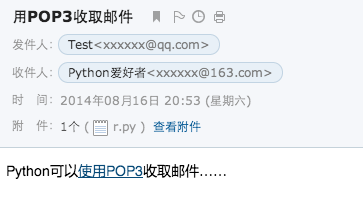
\includegraphics[width=0.6\linewidth]{fig/967965753208928.png}
\end{figure}


运行程序,结果如下:

\begin{pythoncode}
+OK Welcome to coremail Mail Pop3 Server (163coms[...])
Messages: 126. Size: 27228317

From: Test <xxxxxx@qq.com>
To: Python爱好者 <xxxxxx@163.com>
Subject: 用POP3收取邮件
part 0
--------------------
  part 0
  --------------------
    Text: Python可以使用POP3收取邮件……...
  part 1
  --------------------
    Text: Python可以<a href="...">使用POP3</a>收取邮件……...
part 1
--------------------
  Attachment: application/octet-stream
\end{pythoncode}

我们从打印的结构可以看出,这封邮件是一个\texttt{MIMEMultipart},它包含两部分:第一部分又是一个\texttt{MIMEMultipart},第二部分是一个附件。而内嵌的\texttt{MIMEMultipart}是一个\texttt{alternative}类型,它包含一个纯文本格式的\texttt{MIMEText}和一个
HTML 格式的\texttt{MIMEText}。

\hypertarget{ux5c0fux7ed3}{%
\subsubsection{小结}\label{ux5c0fux7ed3}}

用 Python 的\texttt{poplib}模块收取邮件分两步:第一步是用 POP3
协议把邮件获取到本地,第二步是用\texttt{email}模块把原始邮件解析为\texttt{Message}对象,然后,用适当的形式把邮件内容展示给用户即可。

\hypertarget{ux53c2ux8003ux6e90ux7801}{%
\subsubsection{参考源码}\label{ux53c2ux8003ux6e90ux7801}}

\href{https://github.com/michaelliao/learn-python3/blob/master/samples/mail/fetch_mail.py}{fetch\_mail.py}

